% Options for packages loaded elsewhere
\PassOptionsToPackage{unicode}{hyperref}
\PassOptionsToPackage{hyphens}{url}
\PassOptionsToPackage{dvipsnames,svgnames,x11names}{xcolor}
%
\documentclass[
  letterpaper,
  DIV=11,
  numbers=noendperiod]{scrartcl}

\usepackage{amsmath,amssymb}
\usepackage{iftex}
\ifPDFTeX
  \usepackage[T2A]{fontenc}
  \usepackage[utf8]{inputenc}
  \usepackage{textcomp} % provide euro and other symbols
\else % if luatex or xetex
  \usepackage{unicode-math}
  \defaultfontfeatures{Scale=MatchLowercase}
  \defaultfontfeatures[\rmfamily]{Ligatures=TeX,Scale=1}
\fi
\usepackage{lmodern}
\ifPDFTeX\else  
    % xetex/luatex font selection
  \setmainfont[]{CMU Serif}
  \setsansfont[]{CMU Serif}
  \setmonofont[]{CMU Serif}
\fi
% Use upquote if available, for straight quotes in verbatim environments
\IfFileExists{upquote.sty}{\usepackage{upquote}}{}
\IfFileExists{microtype.sty}{% use microtype if available
  \usepackage[]{microtype}
  \UseMicrotypeSet[protrusion]{basicmath} % disable protrusion for tt fonts
}{}
\makeatletter
\@ifundefined{KOMAClassName}{% if non-KOMA class
  \IfFileExists{parskip.sty}{%
    \usepackage{parskip}
  }{% else
    \setlength{\parindent}{0pt}
    \setlength{\parskip}{6pt plus 2pt minus 1pt}}
}{% if KOMA class
  \KOMAoptions{parskip=half}}
\makeatother
\usepackage{xcolor}
\setlength{\emergencystretch}{3em} % prevent overfull lines
\setcounter{secnumdepth}{-\maxdimen} % remove section numbering
% Make \paragraph and \subparagraph free-standing
\ifx\paragraph\undefined\else
  \let\oldparagraph\paragraph
  \renewcommand{\paragraph}[1]{\oldparagraph{#1}\mbox{}}
\fi
\ifx\subparagraph\undefined\else
  \let\oldsubparagraph\subparagraph
  \renewcommand{\subparagraph}[1]{\oldsubparagraph{#1}\mbox{}}
\fi


\providecommand{\tightlist}{%
  \setlength{\itemsep}{0pt}\setlength{\parskip}{0pt}}\usepackage{longtable,booktabs,array}
\usepackage{calc} % for calculating minipage widths
% Correct order of tables after \paragraph or \subparagraph
\usepackage{etoolbox}
\makeatletter
\patchcmd\longtable{\par}{\if@noskipsec\mbox{}\fi\par}{}{}
\makeatother
% Allow footnotes in longtable head/foot
\IfFileExists{footnotehyper.sty}{\usepackage{footnotehyper}}{\usepackage{footnote}}
\makesavenoteenv{longtable}
\usepackage{graphicx}
\makeatletter
\def\maxwidth{\ifdim\Gin@nat@width>\linewidth\linewidth\else\Gin@nat@width\fi}
\def\maxheight{\ifdim\Gin@nat@height>\textheight\textheight\else\Gin@nat@height\fi}
\makeatother
% Scale images if necessary, so that they will not overflow the page
% margins by default, and it is still possible to overwrite the defaults
% using explicit options in \includegraphics[width, height, ...]{}
\setkeys{Gin}{width=\maxwidth,height=\maxheight,keepaspectratio}
% Set default figure placement to htbp
\makeatletter
\def\fps@figure{htbp}
\makeatother

\KOMAoption{captions}{tablesignature}
\usepackage[authordate, abbreviate = true, date = year, autocite=inline, backref = true]{biblatex-chicago}
\usepackage{csquotes}
\setlength{\bibhang}{0pt}
\makeatletter
\makeatother
\makeatletter
\makeatother
\makeatletter
\@ifpackageloaded{caption}{}{\usepackage{caption}}
\AtBeginDocument{%
\ifdefined\contentsname
  \renewcommand*\contentsname{Table of contents}
\else
  \newcommand\contentsname{Table of contents}
\fi
\ifdefined\listfigurename
  \renewcommand*\listfigurename{List of Figures}
\else
  \newcommand\listfigurename{List of Figures}
\fi
\ifdefined\listtablename
  \renewcommand*\listtablename{List of Tables}
\else
  \newcommand\listtablename{List of Tables}
\fi
\ifdefined\figurename
  \renewcommand*\figurename{Figure}
\else
  \newcommand\figurename{Figure}
\fi
\ifdefined\tablename
  \renewcommand*\tablename{Table}
\else
  \newcommand\tablename{Table}
\fi
}
\@ifpackageloaded{float}{}{\usepackage{float}}
\floatstyle{ruled}
\@ifundefined{c@chapter}{\newfloat{codelisting}{h}{lop}}{\newfloat{codelisting}{h}{lop}[chapter]}
\floatname{codelisting}{Listing}
\newcommand*\listoflistings{\listof{codelisting}{List of Listings}}
\makeatother
\makeatletter
\@ifpackageloaded{caption}{}{\usepackage{caption}}
\@ifpackageloaded{subcaption}{}{\usepackage{subcaption}}
\makeatother
\makeatletter
\@ifpackageloaded{tcolorbox}{}{\usepackage[skins,breakable]{tcolorbox}}
\makeatother
\makeatletter
\@ifundefined{shadecolor}{\definecolor{shadecolor}{rgb}{.97, .97, .97}}
\makeatother
\makeatletter
\makeatother
\makeatletter
\makeatother
\ifLuaTeX
\usepackage[bidi=basic]{babel}
\else
\usepackage[bidi=default]{babel}
\fi
\babelprovide[main,import]{english}
% get rid of language-specific shorthands (see #6817):
\let\LanguageShortHands\languageshorthands
\def\languageshorthands#1{}
\ifLuaTeX
  \usepackage{selnolig}  % disable illegal ligatures
\fi
\usepackage[]{biblatex}
\addbibresource{bibliography.bib}
\usepackage{csquotes}
\IfFileExists{bookmark.sty}{\usepackage{bookmark}}{\usepackage{hyperref}}
\IfFileExists{xurl.sty}{\usepackage{xurl}}{} % add URL line breaks if available
\urlstyle{same} % disable monospaced font for URLs
\hypersetup{
  pdftitle={Student dropout analysis based on previously acquired educational achievements: A case of the University of Portalegre},
  pdfauthor={Izeldeen Nedal Yunis Al Fraijat; Danat Semeneev; Ieva Žube; Pankaj Chattri; Kristaps Eglītis},
  pdflang={en},
  pdfkeywords={AA1, AA2},
  colorlinks=true,
  linkcolor={blue},
  filecolor={Maroon},
  citecolor={Blue},
  urlcolor={Blue},
  pdfcreator={LaTeX via pandoc}}

\title{Student dropout analysis based on previously acquired educational
achievements: A case of the University of Portalegre}
\usepackage{etoolbox}
\makeatletter
\providecommand{\subtitle}[1]{% add subtitle to \maketitle
  \apptocmd{\@title}{\par {\large #1 \par}}{}{}
}
\makeatother
\subtitle{Business Analysis, Business Informatics Ms, Fall 2023.}
\author{Izeldeen Nedal Yunis Al Fraijat \and Danat Semeneev \and Ieva
Žube \and Pankaj Chattri \and Kristaps Eglītis\footnote{Rīga Technical
  University}}
\date{2023-12-11}

\begin{document}
\maketitle
\begin{abstract}
.
\end{abstract}
\ifdefined\Shaded\renewenvironment{Shaded}{\begin{tcolorbox}[boxrule=0pt, frame hidden, interior hidden, breakable, sharp corners, enhanced, borderline west={3pt}{0pt}{shadecolor}]}{\end{tcolorbox}}\fi

\hypertarget{abstract}{%
\subsection{Abstract}\label{abstract}}

In the world of education, the path to success is often visualized as a
linear progression, where students follow a predefined journey from
kindergarten to graduation. However, the reality is far more complex.
Various reasons lead students to choose to deviate from this path. These
students have encountered different challenges, circumstances, or a lack
of proper resources that have led them to drop out of university.

In this dataset provided to us, we will delve deeper into understanding
the reasons why students have dropped out of the university, based on
the data at our disposal. We will leverage our social knowledge to
comprehend the factors that influenced their decision to drop out and
work to prevent such occurrences if the issues are within the
university's purview. Our goal is to offer solutions, support, and the
necessary resources to facilitate students' educational journeys. We
will also use the analysis we've conducted on the dropout students to
learn from their experiences and chart a unique educational pathway with
fewer dropouts.

\hypertarget{introduction}{%
\section{Introduction}\label{introduction}}

Starting from preliminary school we are told that having an education is
very important for your future or that without higher education your job
possibilities are going to be very limited. While primary education is
mandatory, having higher education is not. But why do people actually
take their time and resources to pursue it? Well, according to studies
the most important factor for pursuing higher education is job
acquisition. \autocite{knutsen_motivation_2011} Some other factors may
include increased income in the existing job, improved work conditions
or increased ability for retirement. All in all they do all tie up to
materialistic benefits in the end. Of course, other, more intrisic
factors include seeking for additional knowledge or self-fulfillment
\autocite{cortes_factors_2023}. There are also factors like meeting new
friends, improving social interaction skills or just wanting to make a
difference in the world. Of course factors that cannot be ignored are
social pressure \autocite{temple_factors_2009}, meaning that having
friends that want to pursue higher education can influence ones own
decision or influence of family members. Pursuing higher edication is
good, but what about people who prematurely end their studies and drop
out? What could be the factors that lead to such a decision? Based on
the study and datasets that we used for our research there are multiple
factors that influence dropping out.

Nevertheless, pursuing higher education and actually getting the degree
has some tangible benefits. According to an OECD -- Education at a
Glance 2019 research paper \autocite{oecd_education_2019}, \enquote{On
average across OECD countries, adults with a short-cycle tertiary degree
earn 20\% more than adults with upper secondary education. The earnings
advantage increases to 44\% for those with a bachelor's degree and to
91\% for those with a master's or doctorPal degree.} With this in mind,
it is important for government and educational institutions to ensure
high level of graduates in society to ensure economic growth and overall
increase in well-being. To measure the success of this goal, it is
important to set KPI's, track them and make educated conclusions on what
needs to be done or is being done right to reach the goal of higher
educated society.

\hypertarget{target-metrics-and-kpi}{%
\subsection{Target Metrics and KPI}\label{target-metrics-and-kpi}}

In this particular case, KPI's will be chosen based on datasets of
Portugese High Schools but most likely data can be generalised, atleast
for Europe, as the region and sociodemographics are not so different.
Even though there are many factors that influence the success of
graduation, only factors that can be proven by government and
educational institutions will be chosen. After rigorous analysis, we
propose the following grades.

\begin{enumerate}
\def\labelenumi{\arabic{enumi}.}
\item
  Academic support. Based on the dataset students who had support had 3x
  lower dropout rates than students that didn't have. This means that
  governments should be incentivised to allocate a higher amount of
  budget towards education to give financial aid and motivate students
  to complete their studies.
\item
  Institutional improvements. Again, based on datasets, schools with
  improvements have 40\% less dropout rate than schools without. This is
  something that can be improved by incentivizing teachers with higher
  salaries or giving schools more budget to improve their workstations.
\item
  Student grades. Datasets tell us that the higher the average grade,
  the lower the dropout rate. Usually students that have low grades are
  uninterested in the subjects which could be due to having chosen not
  the right program for them or that the way lectures and information is
  presented is uninteresting or outdated. Either way this can be
  improved. Increasing the possibility that the student has chosen the
  right program for him can be done by introducing more \enquote{open
  days} in higher education institutions and having more upfront
  information about what can be expected from programs. The overall
  lecture performance can be improved by taking more time to have
  up-to-date information presented and teachers having decent motivation
  of teaching students. This can be achieved by increasing teacher
  salaries and institutions having more control over teachers and
  information they present to students.
\end{enumerate}

\hypertarget{exploratory-data-analysis}{%
\subsection{Exploratory Data Analysis}\label{exploratory-data-analysis}}

\hypertarget{descriptive-statistics}{%
\subsubsection{Descriptive Statistics}\label{descriptive-statistics}}

\hypertarget{tab-example}{}
\begin{longtable}[]{@{}ll@{}}
\toprule\noalign{}
& Data Type \\
\midrule\noalign{}
\endfirsthead
\toprule\noalign{}
& Data Type \\
\midrule\noalign{}
\endhead
\bottomrule\noalign{}
\endlastfoot
Marital status & int64 \\
Application mode & int64 \\
Application order & int64 \\
Course & int64 \\
Daytime/evening attendance & int64 \\
Previous qualification & int64 \\
Previous qualification (grade) & float64 \\
Nacionality & int64 \\
Mother\textquotesingle s qualification & int64 \\
Father\textquotesingle s qualification & int64 \\
Mother\textquotesingle s occupation & int64 \\
Father\textquotesingle s occupation & int64 \\
Admission grade & float64 \\
Displaced & int64 \\
Educational special needs & int64 \\
Debtor & int64 \\
Tuition fees up to date & int64 \\
Gender & int64 \\
Scholarship holder & int64 \\
Age at enrollment & int64 \\
International & int64 \\
Curricular units 1st sem (credited) & int64 \\
Curricular units 1st sem (enrolled) & int64 \\
Curricular units 1st sem (evaluations) & int64 \\
Curricular units 1st sem (approved) & int64 \\
Curricular units 1st sem (grade) & float64 \\
Curricular units 1st sem (without evaluations) & int64 \\
Curricular units 2nd sem (credited) & int64 \\
Curricular units 2nd sem (enrolled) & int64 \\
Curricular units 2nd sem (evaluations) & int64 \\
Curricular units 2nd sem (approved) & int64 \\
Curricular units 2nd sem (grade) & float64 \\
Curricular units 2nd sem (without evaluations) & int64 \\
Unemployment rate & float64 \\
Inflation rate & float64 \\
GDP & float64 \\
Target & object \\
\caption{The data types of the datast columns }\tabularnewline
\end{longtable}

As we have checked, the dataset does not have zero values, so there is
nothing to purge inside it. Later on, we get the basic descriptive
statistics, shown below.

\hypertarget{tab-descstat-1}{}
\begin{longtable}[]{@{}llllll@{}}
\toprule\noalign{}
& Marital status & Application mode & Application order & Course &
Daytime/evening attendance \\
\midrule\noalign{}
\endfirsthead
\toprule\noalign{}
& Marital status & Application mode & Application order & Course &
Daytime/evening attendance \\
\midrule\noalign{}
\endhead
\bottomrule\noalign{}
\endlastfoot
count & 4424.000000 & 4424.000000 & 4424.000000 & 4424.000000 &
4424.000000 \\
mean & 1.178571 & 18.669078 & 1.727848 & 8856.642631 & 0.890823 \\
std & 0.605747 & 17.484682 & 1.313793 & 2063.566416 & 0.311897 \\
min & 1.000000 & 1.000000 & 0.000000 & 33.000000 & 0.000000 \\
25\% & 1.000000 & 1.000000 & 1.000000 & 9085.000000 & 1.000000 \\
50\% & 1.000000 & 17.000000 & 1.000000 & 9238.000000 & 1.000000 \\
75\% & 1.000000 & 39.000000 & 2.000000 & 9556.000000 & 1.000000 \\
max & 6.000000 & 57.000000 & 9.000000 & 9991.000000 & 1.000000 \\
\caption{Descriptive statistics }\tabularnewline
\end{longtable}

\hypertarget{tab-descstat-2}{}
\begin{longtable}[]{@{}llllll@{}}
\toprule\noalign{}
& Previous qualification & Previous qualification (grade) & Nacionality
& Mother\textquotesingle s qualification & Father\textquotesingle s
qualification \\
\midrule\noalign{}
\endfirsthead
\toprule\noalign{}
& Previous qualification & Previous qualification (grade) & Nacionality
& Mother\textquotesingle s qualification & Father\textquotesingle s
qualification \\
\midrule\noalign{}
\endhead
\bottomrule\noalign{}
\endlastfoot
count & 4424.000000 & 4424.000000 & 4424.000000 & 4424.000000 &
4424.000000 \\
mean & 4.577758 & 132.613314 & 1.873192 & 19.561935 & 22.275316 \\
std & 10.216592 & 13.188332 & 6.914514 & 15.603186 & 15.343108 \\
min & 1.000000 & 95.000000 & 1.000000 & 1.000000 & 1.000000 \\
25\% & 1.000000 & 125.000000 & 1.000000 & 2.000000 & 3.000000 \\
50\% & 1.000000 & 133.100000 & 1.000000 & 19.000000 & 19.000000 \\
75\% & 1.000000 & 140.000000 & 1.000000 & 37.000000 & 37.000000 \\
max & 43.000000 & 190.000000 & 109.000000 & 44.000000 & 44.000000 \\
\caption{Descriptive statistics (cont'd) }\tabularnewline
\end{longtable}

\hypertarget{tab-descstat-3}{}
\begin{longtable}[]{@{}llllll@{}}
\toprule\noalign{}
& Mother\textquotesingle s occupation & Father\textquotesingle s
occupation & Admission grade & Displaced & Educational special needs \\
\midrule\noalign{}
\endfirsthead
\toprule\noalign{}
& Mother\textquotesingle s occupation & Father\textquotesingle s
occupation & Admission grade & Displaced & Educational special needs \\
\midrule\noalign{}
\endhead
\bottomrule\noalign{}
\endlastfoot
count & 4424.000000 & 4424.000000 & 4424.000000 & 4424.000000 &
4424.000000 \\
mean & 10.960895 & 11.032324 & 126.978119 & 0.548373 & 0.011528 \\
std & 26.418253 & 25.263040 & 14.482001 & 0.497711 & 0.106760 \\
min & 0.000000 & 0.000000 & 95.000000 & 0.000000 & 0.000000 \\
25\% & 4.000000 & 4.000000 & 117.900000 & 0.000000 & 0.000000 \\
50\% & 5.000000 & 7.000000 & 126.100000 & 1.000000 & 0.000000 \\
75\% & 9.000000 & 9.000000 & 134.800000 & 1.000000 & 0.000000 \\
max & 194.000000 & 195.000000 & 190.000000 & 1.000000 & 1.000000 \\
\caption{Descriptive statistics (cont'd) }\tabularnewline
\end{longtable}

\hypertarget{tab-descstat-4}{}
\begin{longtable}[]{@{}llllll@{}}
\toprule\noalign{}
& Debtor & Tuition fees up to date & Gender & Scholarship holder & Age
at enrollment \\
\midrule\noalign{}
\endfirsthead
\toprule\noalign{}
& Debtor & Tuition fees up to date & Gender & Scholarship holder & Age
at enrollment \\
\midrule\noalign{}
\endhead
\bottomrule\noalign{}
\endlastfoot
count & 4424.000000 & 4424.000000 & 4424.000000 & 4424.000000 &
4424.000000 \\
mean & 0.113698 & 0.880651 & 0.351718 & 0.248418 & 23.265145 \\
std & 0.317480 & 0.324235 & 0.477560 & 0.432144 & 7.587816 \\
min & 0.000000 & 0.000000 & 0.000000 & 0.000000 & 17.000000 \\
25\% & 0.000000 & 1.000000 & 0.000000 & 0.000000 & 19.000000 \\
50\% & 0.000000 & 1.000000 & 0.000000 & 0.000000 & 20.000000 \\
75\% & 0.000000 & 1.000000 & 1.000000 & 0.000000 & 25.000000 \\
max & 1.000000 & 1.000000 & 1.000000 & 1.000000 & 70.000000 \\
\caption{Descriptive statistics (cont'd) }\tabularnewline
\end{longtable}

\hypertarget{tab-descstat-5}{}
\begin{longtable}[]{@{}lllll@{}}
\toprule\noalign{}
& International & Curricular units 1st sem (credited) & Curricular units
1st sem (enrolled) & Curricular units 1st sem (evaluations) \\
\midrule\noalign{}
\endfirsthead
\toprule\noalign{}
& International & Curricular units 1st sem (credited) & Curricular units
1st sem (enrolled) & Curricular units 1st sem (evaluations) \\
\midrule\noalign{}
\endhead
\bottomrule\noalign{}
\endlastfoot
count & 4424.000000 & 4424.000000 & 4424.000000 & 4424.000000 \\
mean & 0.024864 & 0.709991 & 6.270570 & 8.299051 \\
std & 0.155729 & 2.360507 & 2.480178 & 4.179106 \\
min & 0.000000 & 0.000000 & 0.000000 & 0.000000 \\
25\% & 0.000000 & 0.000000 & 5.000000 & 6.000000 \\
50\% & 0.000000 & 0.000000 & 6.000000 & 8.000000 \\
75\% & 0.000000 & 0.000000 & 7.000000 & 10.000000 \\
max & 1.000000 & 20.000000 & 26.000000 & 45.000000 \\
\caption{Descriptive statistics (cont'd) }\tabularnewline
\end{longtable}

\hypertarget{tab-descstat-6}{}
\begin{longtable}[]{@{}lllll@{}}
\toprule\noalign{}
& Curricular units 1st sem (approved) & Curricular units 1st sem (grade)
& Curricular units 1st sem (without evaluations) & Curricular units 2nd
sem (credited) \\
\midrule\noalign{}
\endfirsthead
\toprule\noalign{}
& Curricular units 1st sem (approved) & Curricular units 1st sem (grade)
& Curricular units 1st sem (without evaluations) & Curricular units 2nd
sem (credited) \\
\midrule\noalign{}
\endhead
\bottomrule\noalign{}
\endlastfoot
count & 4424.000000 & 4424.000000 & 4424.000000 & 4424.000000 \\
mean & 4.706600 & 10.640822 & 0.137658 & 0.541817 \\
std & 3.094238 & 4.843663 & 0.690880 & 1.918546 \\
min & 0.000000 & 0.000000 & 0.000000 & 0.000000 \\
25\% & 3.000000 & 11.000000 & 0.000000 & 0.000000 \\
50\% & 5.000000 & 12.285714 & 0.000000 & 0.000000 \\
75\% & 6.000000 & 13.400000 & 0.000000 & 0.000000 \\
max & 26.000000 & 18.875000 & 12.000000 & 19.000000 \\
\caption{Descriptive statistics (cont'd) }\tabularnewline
\end{longtable}

\hypertarget{tab-descstat-7}{}
\begin{longtable}[]{@{}lllll@{}}
\toprule\noalign{}
& Curricular units 2nd sem (enrolled) & Curricular units 2nd sem
(evaluations) & Curricular units 2nd sem (approved) & Curricular units
2nd sem (grade) \\
\midrule\noalign{}
\endfirsthead
\toprule\noalign{}
& Curricular units 2nd sem (enrolled) & Curricular units 2nd sem
(evaluations) & Curricular units 2nd sem (approved) & Curricular units
2nd sem (grade) \\
\midrule\noalign{}
\endhead
\bottomrule\noalign{}
\endlastfoot
count & 4424.000000 & 4424.000000 & 4424.000000 & 4424.000000 \\
mean & 6.232143 & 8.063291 & 4.435805 & 10.230206 \\
std & 2.195951 & 3.947951 & 3.014764 & 5.210808 \\
min & 0.000000 & 0.000000 & 0.000000 & 0.000000 \\
25\% & 5.000000 & 6.000000 & 2.000000 & 10.750000 \\
50\% & 6.000000 & 8.000000 & 5.000000 & 12.200000 \\
75\% & 7.000000 & 10.000000 & 6.000000 & 13.333333 \\
max & 23.000000 & 33.000000 & 20.000000 & 18.571429 \\
\caption{Descriptive statistics (cont'd) }\tabularnewline
\end{longtable}

The students are from multiple countries, but the overwhelming majority
of the students are from Portugal. It would be interesting to see how
the students' admission grade depends on their previous qualification,
particularily because of that many students from abroad are from the
Ultramarine Territories where it's more challenging to get comparable
education.

\begin{longtable}[]{@{}llllllllllllllllllllll@{}}
\toprule\noalign{}
& Marital status & Application mode & Application order & Course &
Daytime/evening attendance & Previous qualification & Previous
qualification (grade) & Nacionality & Mother\textquotesingle s
qualification & Father\textquotesingle s qualification & ... &
Curricular units 2nd sem (credited) & Curricular units 2nd sem
(enrolled) & Curricular units 2nd sem (evaluations) & Curricular units
2nd sem (approved) & Curricular units 2nd sem (grade) & Curricular units
2nd sem (without evaluations) & Unemployment rate & Inflation rate & GDP
& Target \\
\midrule\noalign{}
\endhead
\bottomrule\noalign{}
\endlastfoot
0 & 1 & 17 & 5 & 171 & 1 & 1 & 122.0 & 1 & 19 & 12 & ... & 0 & 0 & 0 & 0
& 0.000000 & 0 & 10.8 & 1.4 & 1.74 & Dropout \\
1 & 1 & 15 & 1 & 9254 & 1 & 1 & 160.0 & 1 & 1 & 3 & ... & 0 & 6 & 6 & 6
& 13.666667 & 0 & 13.9 & -0.3 & 0.79 & Graduate \\
2 & 1 & 1 & 5 & 9070 & 1 & 1 & 122.0 & 1 & 37 & 37 & ... & 0 & 6 & 0 & 0
& 0.000000 & 0 & 10.8 & 1.4 & 1.74 & Dropout \\
3 & 1 & 17 & 2 & 9773 & 1 & 1 & 122.0 & 1 & 38 & 37 & ... & 0 & 6 & 10 &
5 & 12.400000 & 0 & 9.4 & -0.8 & -3.12 & Graduate \\
4 & 2 & 39 & 1 & 8014 & 0 & 1 & 100.0 & 1 & 37 & 38 & ... & 0 & 6 & 6 &
6 & 13.000000 & 0 & 13.9 & -0.3 & 0.79 & Graduate \\
... & ... & ... & ... & ... & ... & ... & ... & ... & ... & ... & ... &
... & ... & ... & ... & ... & ... & ... & ... & ... & ... \\
4419 & 1 & 1 & 6 & 9773 & 1 & 1 & 125.0 & 1 & 1 & 1 & ... & 0 & 6 & 8 &
5 & 12.666667 & 0 & 15.5 & 2.8 & -4.06 & Graduate \\
4420 & 1 & 1 & 2 & 9773 & 1 & 1 & 120.0 & 105 & 1 & 1 & ... & 0 & 6 & 6
& 2 & 11.000000 & 0 & 11.1 & 0.6 & 2.02 & Dropout \\
4421 & 1 & 1 & 1 & 9500 & 1 & 1 & 154.0 & 1 & 37 & 37 & ... & 0 & 8 & 9
& 1 & 13.500000 & 0 & 13.9 & -0.3 & 0.79 & Dropout \\
4422 & 1 & 1 & 1 & 9147 & 1 & 1 & 180.0 & 1 & 37 & 37 & ... & 0 & 5 & 6
& 5 & 12.000000 & 0 & 9.4 & -0.8 & -3.12 & Graduate \\
4423 & 1 & 10 & 1 & 9773 & 1 & 1 & 152.0 & 22 & 38 & 37 & ... & 0 & 6 &
6 & 6 & 13.000000 & 0 & 12.7 & 3.7 & -1.70 & Graduate \\
\end{longtable}

\begin{verbatim}
Series([], Name: Previous qualification (grade), dtype: float64)
\end{verbatim}

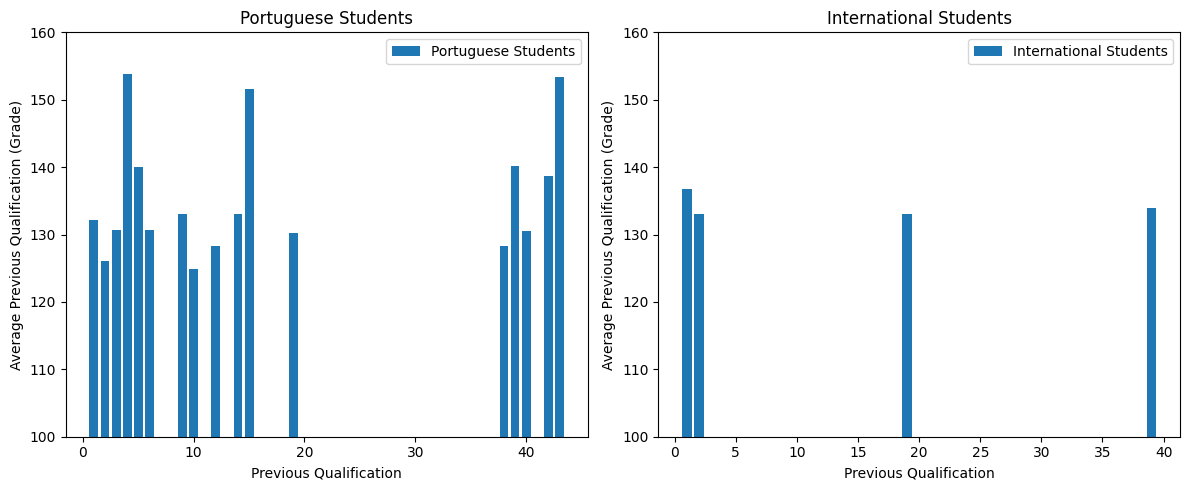
\includegraphics{report_AzadhdhinNedalYunisAlFraijat_files/figure-pdf/cell-17-output-1.png}

Also, there is a drastic imbalance over yet another crucial factor: age.
As it was mentioned previously, students of age are far less ubiquitous,
can have far more incentives to abandon studies and with smaller
potential to apprehension of material. Indeed, this is eloquently
manifested on the next graph.

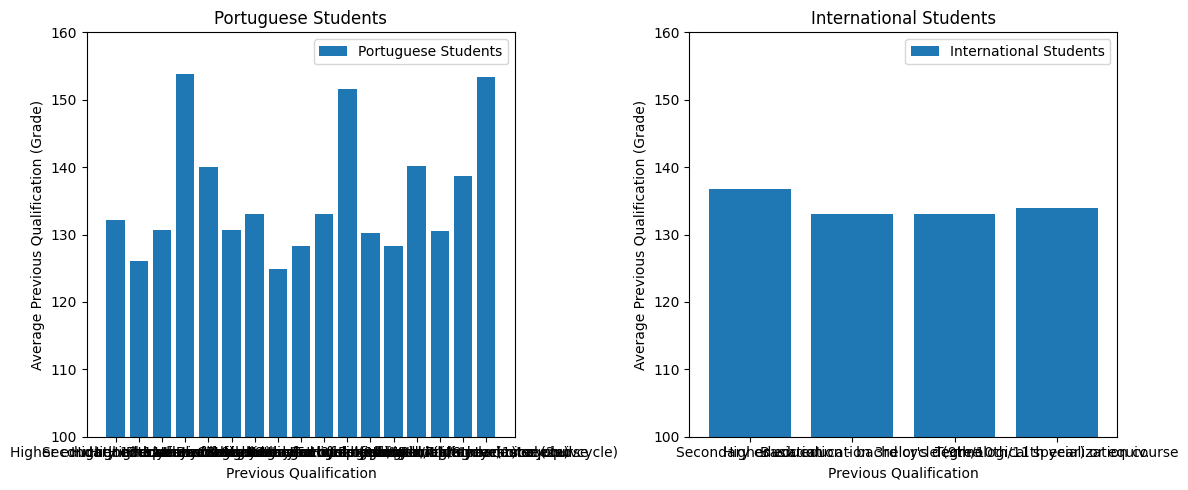
\includegraphics{report_AzadhdhinNedalYunisAlFraijat_files/figure-pdf/cell-18-output-1.png}

Q. v. the sizes of the bins for dropout students differ far less than
the total size for the name of the student.

If the hypothesis about some external factors, The target variable
should be much dependent on previous grades,\\
The datapoint cloud, however, shows that this rule has a lot of
exceptions.

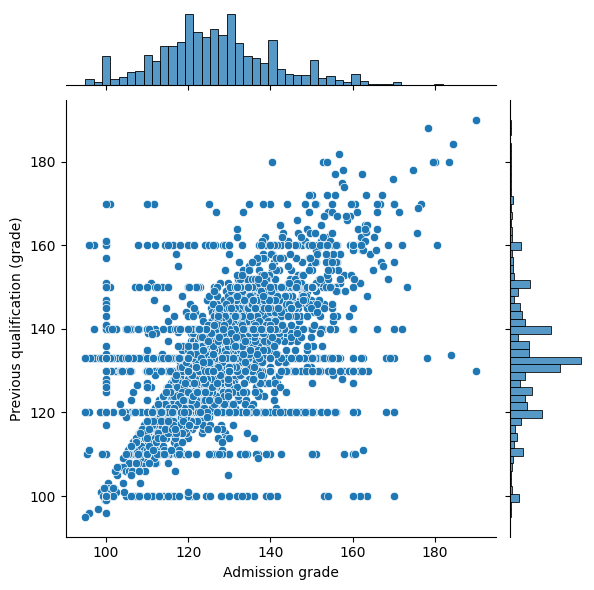
\includegraphics{report_AzadhdhinNedalYunisAlFraijat_files/figure-pdf/cell-20-output-1.png}

We can draw the following observations:

\begin{itemize}
\item
  The \textbf{distribution of admission grades} is roughly normal with
  most students scoring between \textbf{\emph{60 to 80 marks}}.
\item
  The \textbf{distribution of previous qualifications} (grades) is also
  the same with most of them having grades in between \textbf{\emph{12
  and 16}}.
\item
  There is seen a \textbf{positive correlation} between admission grade
  and previous qualification grade indicating students with higher
  previous qualifications tend to have higher admission grades.
\end{itemize}

In the previous graphs, we considered qualitative columns that are more
or less exogenous to the dataset.

However, the majority of columns of this dataset are qualitative and
they do not much fit, so we would opt for analysis of discriminate
groups. This was the visualization for the few quantitative columns,
which shows the natural interconnection between the curricularly accrued
units in the 1st and the 2nd year, which are in turn mostly unrelated to
the admission grade. This is understandable since the grades are
commonly based on the successfulness of the local program and student's
toil, while the students backgrounds are commonly different and this
puts them into inequitable positions when passing the admission exams.

We also consider the impact of scholarships and other compensations in
academic support, which should quench the complications associated with
adaptations in new environment.

\begin{verbatim}
Text(0.5, 1.0, 'Influence of Socioeconomic Factors on Dropout Rates')
\end{verbatim}

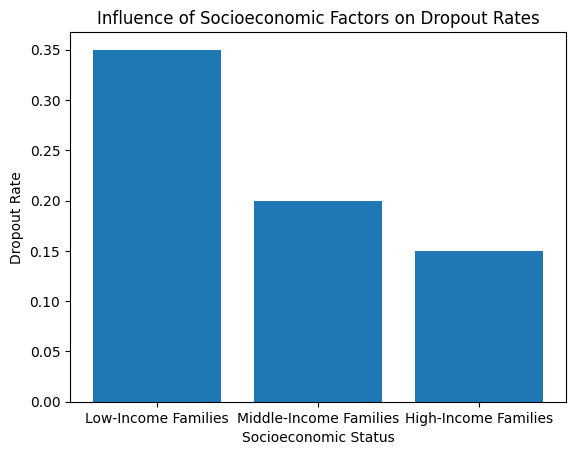
\includegraphics{report_AzadhdhinNedalYunisAlFraijat_files/figure-pdf/cell-21-output-2.png}

\textbf{Observations :}

\begin{itemize}
\tightlist
\item
  Students coming from \emph{low - income families have a higher dropout
  rate} than compared from middle - income and high - income families.
\end{itemize}

Furthermore, not only the pecuniary, but also institutional aspects can
be improved -- and so influence the academic success. Below we
demonstrate how the institutional improvements can influence the
dropout.

\begin{verbatim}
Text(0.5, 1.0, 'Effect of Institutional Improvements on Student Retention')
\end{verbatim}

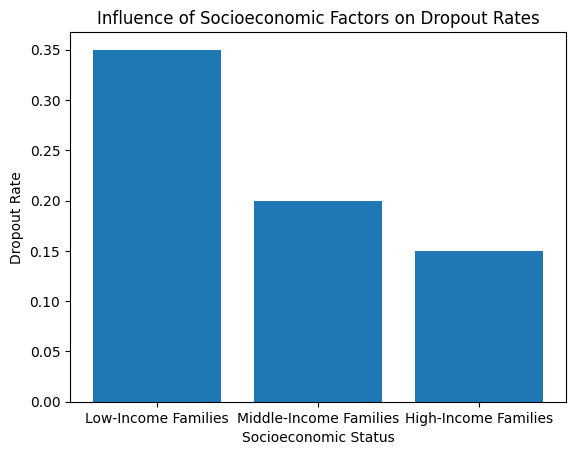
\includegraphics{report_AzadhdhinNedalYunisAlFraijat_files/figure-pdf/cell-22-output-2.png}

\textbf{Observations :}

\begin{itemize}
\tightlist
\item
  Schools having \emph{implemented institutional improvements yeilds a
  significant lowering of the dropout rate} when compared to those
  without.
\end{itemize}

In different studies, it is quite common to compare the academic success
of a student with the academic successes of ttheir parents as this has
both direct and indirect effects , s. a. i. e. both are connected to
welfare, but also it can be that there is another channel of knowledge
transmission to the younger generation.

\begin{verbatim}
Text(0.5, 1.0, "Influence of Mother's Occupation on Dropout Rates")
\end{verbatim}

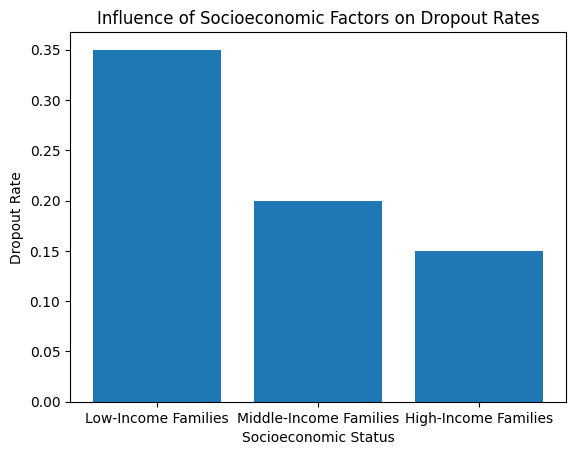
\includegraphics{report_AzadhdhinNedalYunisAlFraijat_files/figure-pdf/cell-23-output-2.png}

\textbf{Observations :}

\begin{itemize}
\item
  The bar chart shows that \emph{Students with mothers in lower-level
  occupations} tend to have higher dropout rates than compared to those
  with mothers in high paying jobs.
\item
  This also may suggest the mother's occupation can influence student
  retention, emphasizing the need for financial support and family
  engagement.
\end{itemize}

\begin{verbatim}
Collecting plotly
  Using cached plotly-5.18.0-py3-none-any.whl (15.6 MB)
Collecting tenacity>=6.2.0
  Using cached tenacity-8.2.3-py3-none-any.whl (24 kB)
Requirement already satisfied: packaging in /Users/romulaperov/.pyenv/versions/3.11.1/lib/python3.11/site-packages (from plotly) (23.2)
Installing collected packages: tenacity, plotly
Successfully installed plotly-5.18.0 tenacity-8.2.3

[notice] A new release of pip available: 22.3.1 -> 23.3.1
[notice] To update, run: pip install --upgrade pip
\end{verbatim}

\begin{verbatim}
Requirement already satisfied: pandas in /opt/homebrew/Caskroom/miniconda/base/lib/python3.11/site-packages (1.5.3)
Requirement already satisfied: scikit-learn in /opt/homebrew/Caskroom/miniconda/base/lib/python3.11/site-packages (1.2.2)
Requirement already satisfied: plotly in /opt/homebrew/Caskroom/miniconda/base/lib/python3.11/site-packages (5.17.0)
Requirement already satisfied: python-dateutil>=2.8.1 in /opt/homebrew/Caskroom/miniconda/base/lib/python3.11/site-packages (from pandas) (2.8.2)
Requirement already satisfied: pytz>=2020.1 in /opt/homebrew/Caskroom/miniconda/base/lib/python3.11/site-packages (from pandas) (2023.3.post1)
Requirement already satisfied: numpy>=1.21.0 in /opt/homebrew/Caskroom/miniconda/base/lib/python3.11/site-packages (from pandas) (1.25.2)
Requirement already satisfied: scipy>=1.3.2 in /opt/homebrew/Caskroom/miniconda/base/lib/python3.11/site-packages (from scikit-learn) (1.10.1)
Requirement already satisfied: joblib>=1.1.1 in /opt/homebrew/Caskroom/miniconda/base/lib/python3.11/site-packages (from scikit-learn) (1.3.2)
Requirement already satisfied: threadpoolctl>=2.0.0 in /opt/homebrew/Caskroom/miniconda/base/lib/python3.11/site-packages (from scikit-learn) (3.2.0)
Requirement already satisfied: tenacity>=6.2.0 in /opt/homebrew/Caskroom/miniconda/base/lib/python3.11/site-packages (from plotly) (8.2.3)
Requirement already satisfied: packaging in /opt/homebrew/Caskroom/miniconda/base/lib/python3.11/site-packages (from plotly) (23.1)
Requirement already satisfied: six>=1.5 in /opt/homebrew/Caskroom/miniconda/base/lib/python3.11/site-packages (from python-dateutil>=2.8.1->pandas) (1.16.0)
\end{verbatim}

\begin{verbatim}
/usr/local/bin/pip3
\end{verbatim}

\begin{verbatim}
/opt/homebrew/Caskroom/miniconda/base/bin/python
\end{verbatim}

\begin{verbatim}
ModuleNotFoundError: No module named 'pandas'
\end{verbatim}

\begin{verbatim}
Requirement already satisfied: pycaret in /opt/homebrew/Caskroom/miniconda/base/lib/python3.11/site-packages (3.2.0)
Requirement already satisfied: category-encoders>=2.4.0 in /opt/homebrew/Caskroom/miniconda/base/lib/python3.11/site-packages (from pycaret) (2.6.3)
Requirement already satisfied: cloudpickle in /opt/homebrew/Caskroom/miniconda/base/lib/python3.11/site-packages (from pycaret) (3.0.0)
Requirement already satisfied: deprecation>=2.1.0 in /opt/homebrew/Caskroom/miniconda/base/lib/python3.11/site-packages (from pycaret) (2.1.0)
Requirement already satisfied: imbalanced-learn>=0.8.1 in /opt/homebrew/Caskroom/miniconda/base/lib/python3.11/site-packages (from pycaret) (0.11.0)
Requirement already satisfied: importlib-metadata>=4.12.0 in /opt/homebrew/Caskroom/miniconda/base/lib/python3.11/site-packages (from pycaret) (6.8.0)
Requirement already satisfied: ipython>=5.5.0 in /opt/homebrew/Caskroom/miniconda/base/lib/python3.11/site-packages (from pycaret) (8.15.0)
Requirement already satisfied: ipywidgets>=7.6.5 in /opt/homebrew/Caskroom/miniconda/base/lib/python3.11/site-packages (from pycaret) (8.0.4)
Requirement already satisfied: jinja2>=1.2 in /opt/homebrew/Caskroom/miniconda/base/lib/python3.11/site-packages (from pycaret) (3.1.2)
Requirement already satisfied: joblib>=1.2.0 in /opt/homebrew/Caskroom/miniconda/base/lib/python3.11/site-packages (from pycaret) (1.3.2)
Requirement already satisfied: kaleido>=0.2.1 in /opt/homebrew/Caskroom/miniconda/base/lib/python3.11/site-packages (from pycaret) (0.2.1)
Requirement already satisfied: lightgbm>=3.0.0 in /opt/homebrew/Caskroom/miniconda/base/lib/python3.11/site-packages (from pycaret) (4.1.0)
Requirement already satisfied: markupsafe>=2.0.1 in /opt/homebrew/Caskroom/miniconda/base/lib/python3.11/site-packages (from pycaret) (2.1.1)
Requirement already satisfied: matplotlib<=3.6,>=3.3.0 in /opt/homebrew/Caskroom/miniconda/base/lib/python3.11/site-packages (from pycaret) (3.6.0)
Requirement already satisfied: nbformat>=4.2.0 in /opt/homebrew/Caskroom/miniconda/base/lib/python3.11/site-packages (from pycaret) (5.9.2)
Requirement already satisfied: numba>=0.55.0 in /opt/homebrew/Caskroom/miniconda/base/lib/python3.11/site-packages (from pycaret) (0.58.1)
Requirement already satisfied: numpy<1.27,>=1.21 in /opt/homebrew/Caskroom/miniconda/base/lib/python3.11/site-packages (from pycaret) (1.25.2)
Requirement already satisfied: pandas<2.0.0,>=1.3.0 in /opt/homebrew/Caskroom/miniconda/base/lib/python3.11/site-packages (from pycaret) (1.5.3)
Requirement already satisfied: plotly-resampler>=0.8.3.1 in /opt/homebrew/Caskroom/miniconda/base/lib/python3.11/site-packages (from pycaret) (0.9.1)
Requirement already satisfied: plotly>=5.0.0 in /opt/homebrew/Caskroom/miniconda/base/lib/python3.11/site-packages (from pycaret) (5.17.0)
Requirement already satisfied: pmdarima!=1.8.1,<3.0.0,>=1.8.0 in /opt/homebrew/Caskroom/miniconda/base/lib/python3.11/site-packages (from pycaret) (2.0.4)
Requirement already satisfied: psutil>=5.9.0 in /opt/homebrew/Caskroom/miniconda/base/lib/python3.11/site-packages (from pycaret) (5.9.0)
Requirement already satisfied: pyod>=1.0.8 in /opt/homebrew/Caskroom/miniconda/base/lib/python3.11/site-packages (from pycaret) (1.1.1)
Requirement already satisfied: requests>=2.27.1 in /opt/homebrew/Caskroom/miniconda/base/lib/python3.11/site-packages (from pycaret) (2.31.0)
Requirement already satisfied: schemdraw==0.15 in /opt/homebrew/Caskroom/miniconda/base/lib/python3.11/site-packages (from pycaret) (0.15)
Requirement already satisfied: scikit-learn<1.3.0,>=1.0 in /opt/homebrew/Caskroom/miniconda/base/lib/python3.11/site-packages (from pycaret) (1.2.2)
Requirement already satisfied: scikit-plot>=0.3.7 in /opt/homebrew/Caskroom/miniconda/base/lib/python3.11/site-packages (from pycaret) (0.3.7)
Requirement already satisfied: scipy~=1.10.1 in /opt/homebrew/Caskroom/miniconda/base/lib/python3.11/site-packages (from pycaret) (1.10.1)
Requirement already satisfied: sktime!=0.17.1,!=0.17.2,!=0.18.0,<0.22.0,>=0.16.1 in /opt/homebrew/Caskroom/miniconda/base/lib/python3.11/site-packages (from pycaret) (0.21.1)
Requirement already satisfied: statsmodels>=0.12.1 in /opt/homebrew/Caskroom/miniconda/base/lib/python3.11/site-packages (from pycaret) (0.14.0)
Requirement already satisfied: tbats>=1.1.3 in /opt/homebrew/Caskroom/miniconda/base/lib/python3.11/site-packages (from pycaret) (1.1.3)
Requirement already satisfied: tqdm>=4.62.0 in /opt/homebrew/Caskroom/miniconda/base/lib/python3.11/site-packages (from pycaret) (4.65.0)
Requirement already satisfied: xxhash in /opt/homebrew/Caskroom/miniconda/base/lib/python3.11/site-packages (from pycaret) (3.4.1)
Requirement already satisfied: yellowbrick>=1.4 in /opt/homebrew/Caskroom/miniconda/base/lib/python3.11/site-packages (from pycaret) (1.5)
Requirement already satisfied: wurlitzer in /opt/homebrew/Caskroom/miniconda/base/lib/python3.11/site-packages (from pycaret) (3.0.3)
Requirement already satisfied: patsy>=0.5.1 in /opt/homebrew/Caskroom/miniconda/base/lib/python3.11/site-packages (from category-encoders>=2.4.0->pycaret) (0.5.3)
Requirement already satisfied: packaging in /opt/homebrew/Caskroom/miniconda/base/lib/python3.11/site-packages (from deprecation>=2.1.0->pycaret) (23.1)
Requirement already satisfied: threadpoolctl>=2.0.0 in /opt/homebrew/Caskroom/miniconda/base/lib/python3.11/site-packages (from imbalanced-learn>=0.8.1->pycaret) (3.2.0)
Requirement already satisfied: zipp>=0.5 in /opt/homebrew/Caskroom/miniconda/base/lib/python3.11/site-packages (from importlib-metadata>=4.12.0->pycaret) (3.17.0)
Requirement already satisfied: backcall in /opt/homebrew/Caskroom/miniconda/base/lib/python3.11/site-packages (from ipython>=5.5.0->pycaret) (0.2.0)
Requirement already satisfied: decorator in /opt/homebrew/Caskroom/miniconda/base/lib/python3.11/site-packages (from ipython>=5.5.0->pycaret) (5.1.1)
Requirement already satisfied: jedi>=0.16 in /opt/homebrew/Caskroom/miniconda/base/lib/python3.11/site-packages (from ipython>=5.5.0->pycaret) (0.18.1)
Requirement already satisfied: matplotlib-inline in /opt/homebrew/Caskroom/miniconda/base/lib/python3.11/site-packages (from ipython>=5.5.0->pycaret) (0.1.6)
Requirement already satisfied: pickleshare in /opt/homebrew/Caskroom/miniconda/base/lib/python3.11/site-packages (from ipython>=5.5.0->pycaret) (0.7.5)
Collecting prompt-toolkit!=3.0.37,<3.1.0,>=3.0.30 (from ipython>=5.5.0->pycaret)
  Using cached prompt_toolkit-3.0.41-py3-none-any.whl (385 kB)
Requirement already satisfied: pygments>=2.4.0 in /opt/homebrew/Caskroom/miniconda/base/lib/python3.11/site-packages (from ipython>=5.5.0->pycaret) (2.15.1)
Requirement already satisfied: stack-data in /opt/homebrew/Caskroom/miniconda/base/lib/python3.11/site-packages (from ipython>=5.5.0->pycaret) (0.2.0)
Requirement already satisfied: traitlets>=5 in /opt/homebrew/Caskroom/miniconda/base/lib/python3.11/site-packages (from ipython>=5.5.0->pycaret) (5.7.1)
Requirement already satisfied: pexpect>4.3 in /opt/homebrew/Caskroom/miniconda/base/lib/python3.11/site-packages (from ipython>=5.5.0->pycaret) (4.8.0)
Requirement already satisfied: appnope in /opt/homebrew/Caskroom/miniconda/base/lib/python3.11/site-packages (from ipython>=5.5.0->pycaret) (0.1.2)
Requirement already satisfied: ipykernel>=4.5.1 in /opt/homebrew/Caskroom/miniconda/base/lib/python3.11/site-packages (from ipywidgets>=7.6.5->pycaret) (6.25.0)
Requirement already satisfied: widgetsnbextension~=4.0 in /opt/homebrew/Caskroom/miniconda/base/lib/python3.11/site-packages (from ipywidgets>=7.6.5->pycaret) (4.0.5)
Requirement already satisfied: jupyterlab-widgets~=3.0 in /opt/homebrew/Caskroom/miniconda/base/lib/python3.11/site-packages (from ipywidgets>=7.6.5->pycaret) (3.0.5)
Requirement already satisfied: contourpy>=1.0.1 in /opt/homebrew/Caskroom/miniconda/base/lib/python3.11/site-packages (from matplotlib<=3.6,>=3.3.0->pycaret) (1.1.1)
Requirement already satisfied: cycler>=0.10 in /opt/homebrew/Caskroom/miniconda/base/lib/python3.11/site-packages (from matplotlib<=3.6,>=3.3.0->pycaret) (0.12.0)
Requirement already satisfied: fonttools>=4.22.0 in /opt/homebrew/Caskroom/miniconda/base/lib/python3.11/site-packages (from matplotlib<=3.6,>=3.3.0->pycaret) (4.43.0)
Requirement already satisfied: kiwisolver>=1.0.1 in /opt/homebrew/Caskroom/miniconda/base/lib/python3.11/site-packages (from matplotlib<=3.6,>=3.3.0->pycaret) (1.4.5)
Requirement already satisfied: pillow>=6.2.0 in /opt/homebrew/Caskroom/miniconda/base/lib/python3.11/site-packages (from matplotlib<=3.6,>=3.3.0->pycaret) (9.5.0)
Requirement already satisfied: pyparsing>=2.2.1 in /opt/homebrew/Caskroom/miniconda/base/lib/python3.11/site-packages (from matplotlib<=3.6,>=3.3.0->pycaret) (3.1.1)
Requirement already satisfied: python-dateutil>=2.7 in /opt/homebrew/Caskroom/miniconda/base/lib/python3.11/site-packages (from matplotlib<=3.6,>=3.3.0->pycaret) (2.8.2)
Requirement already satisfied: fastjsonschema in /opt/homebrew/Caskroom/miniconda/base/lib/python3.11/site-packages (from nbformat>=4.2.0->pycaret) (2.16.2)
Requirement already satisfied: jsonschema>=2.6 in /opt/homebrew/Caskroom/miniconda/base/lib/python3.11/site-packages (from nbformat>=4.2.0->pycaret) (4.17.3)
Requirement already satisfied: jupyter-core in /opt/homebrew/Caskroom/miniconda/base/lib/python3.11/site-packages (from nbformat>=4.2.0->pycaret) (5.3.0)
Requirement already satisfied: llvmlite<0.42,>=0.41.0dev0 in /opt/homebrew/Caskroom/miniconda/base/lib/python3.11/site-packages (from numba>=0.55.0->pycaret) (0.41.1)
Requirement already satisfied: pytz>=2020.1 in /opt/homebrew/Caskroom/miniconda/base/lib/python3.11/site-packages (from pandas<2.0.0,>=1.3.0->pycaret) (2023.3.post1)
Requirement already satisfied: tenacity>=6.2.0 in /opt/homebrew/Caskroom/miniconda/base/lib/python3.11/site-packages (from plotly>=5.0.0->pycaret) (8.2.3)
Requirement already satisfied: dash<3.0.0,>=2.11.0 in /opt/homebrew/Caskroom/miniconda/base/lib/python3.11/site-packages (from plotly-resampler>=0.8.3.1->pycaret) (2.14.1)
Requirement already satisfied: orjson<4.0.0,>=3.8.0 in /opt/homebrew/Caskroom/miniconda/base/lib/python3.11/site-packages (from plotly-resampler>=0.8.3.1->pycaret) (3.9.10)
Requirement already satisfied: trace-updater>=0.0.8 in /opt/homebrew/Caskroom/miniconda/base/lib/python3.11/site-packages (from plotly-resampler>=0.8.3.1->pycaret) (0.0.9.1)
Requirement already satisfied: tsdownsample==0.1.2 in /opt/homebrew/Caskroom/miniconda/base/lib/python3.11/site-packages (from plotly-resampler>=0.8.3.1->pycaret) (0.1.2)
Requirement already satisfied: Cython!=0.29.18,!=0.29.31,>=0.29 in /opt/homebrew/Caskroom/miniconda/base/lib/python3.11/site-packages (from pmdarima!=1.8.1,<3.0.0,>=1.8.0->pycaret) (3.0.5)
Requirement already satisfied: urllib3 in /opt/homebrew/Caskroom/miniconda/base/lib/python3.11/site-packages (from pmdarima!=1.8.1,<3.0.0,>=1.8.0->pycaret) (1.26.16)
Requirement already satisfied: setuptools!=50.0.0,>=38.6.0 in /opt/homebrew/Caskroom/miniconda/base/lib/python3.11/site-packages (from pmdarima!=1.8.1,<3.0.0,>=1.8.0->pycaret) (68.2.2)
Requirement already satisfied: six in /opt/homebrew/Caskroom/miniconda/base/lib/python3.11/site-packages (from pyod>=1.0.8->pycaret) (1.16.0)
Requirement already satisfied: charset-normalizer<4,>=2 in /opt/homebrew/Caskroom/miniconda/base/lib/python3.11/site-packages (from requests>=2.27.1->pycaret) (2.0.4)
Requirement already satisfied: idna<4,>=2.5 in /opt/homebrew/Caskroom/miniconda/base/lib/python3.11/site-packages (from requests>=2.27.1->pycaret) (3.4)
Requirement already satisfied: certifi>=2017.4.17 in /opt/homebrew/Caskroom/miniconda/base/lib/python3.11/site-packages (from requests>=2.27.1->pycaret) (2023.7.22)
Requirement already satisfied: deprecated>=1.2.13 in /opt/homebrew/Caskroom/miniconda/base/lib/python3.11/site-packages (from sktime!=0.17.1,!=0.17.2,!=0.18.0,<0.22.0,>=0.16.1->pycaret) (1.2.14)
Requirement already satisfied: scikit-base<0.6.0 in /opt/homebrew/Caskroom/miniconda/base/lib/python3.11/site-packages (from sktime!=0.17.1,!=0.17.2,!=0.18.0,<0.22.0,>=0.16.1->pycaret) (0.5.2)
Requirement already satisfied: Flask<3.1,>=1.0.4 in /opt/homebrew/Caskroom/miniconda/base/lib/python3.11/site-packages (from dash<3.0.0,>=2.11.0->plotly-resampler>=0.8.3.1->pycaret) (3.0.0)
Requirement already satisfied: Werkzeug<3.1 in /opt/homebrew/Caskroom/miniconda/base/lib/python3.11/site-packages (from dash<3.0.0,>=2.11.0->plotly-resampler>=0.8.3.1->pycaret) (3.0.1)
Requirement already satisfied: dash-html-components==2.0.0 in /opt/homebrew/Caskroom/miniconda/base/lib/python3.11/site-packages (from dash<3.0.0,>=2.11.0->plotly-resampler>=0.8.3.1->pycaret) (2.0.0)
Requirement already satisfied: dash-core-components==2.0.0 in /opt/homebrew/Caskroom/miniconda/base/lib/python3.11/site-packages (from dash<3.0.0,>=2.11.0->plotly-resampler>=0.8.3.1->pycaret) (2.0.0)
Requirement already satisfied: dash-table==5.0.0 in /opt/homebrew/Caskroom/miniconda/base/lib/python3.11/site-packages (from dash<3.0.0,>=2.11.0->plotly-resampler>=0.8.3.1->pycaret) (5.0.0)
Requirement already satisfied: typing-extensions>=4.1.1 in /opt/homebrew/Caskroom/miniconda/base/lib/python3.11/site-packages (from dash<3.0.0,>=2.11.0->plotly-resampler>=0.8.3.1->pycaret) (4.7.1)
Requirement already satisfied: retrying in /opt/homebrew/Caskroom/miniconda/base/lib/python3.11/site-packages (from dash<3.0.0,>=2.11.0->plotly-resampler>=0.8.3.1->pycaret) (1.3.4)
Requirement already satisfied: ansi2html in /opt/homebrew/Caskroom/miniconda/base/lib/python3.11/site-packages (from dash<3.0.0,>=2.11.0->plotly-resampler>=0.8.3.1->pycaret) (1.8.0)
Requirement already satisfied: nest-asyncio in /opt/homebrew/Caskroom/miniconda/base/lib/python3.11/site-packages (from dash<3.0.0,>=2.11.0->plotly-resampler>=0.8.3.1->pycaret) (1.5.6)
Requirement already satisfied: wrapt<2,>=1.10 in /opt/homebrew/Caskroom/miniconda/base/lib/python3.11/site-packages (from deprecated>=1.2.13->sktime!=0.17.1,!=0.17.2,!=0.18.0,<0.22.0,>=0.16.1->pycaret) (1.15.0)
Requirement already satisfied: comm>=0.1.1 in /opt/homebrew/Caskroom/miniconda/base/lib/python3.11/site-packages (from ipykernel>=4.5.1->ipywidgets>=7.6.5->pycaret) (0.1.2)
Requirement already satisfied: debugpy>=1.6.5 in /opt/homebrew/Caskroom/miniconda/base/lib/python3.11/site-packages (from ipykernel>=4.5.1->ipywidgets>=7.6.5->pycaret) (1.6.7)
Requirement already satisfied: jupyter-client>=6.1.12 in /opt/homebrew/Caskroom/miniconda/base/lib/python3.11/site-packages (from ipykernel>=4.5.1->ipywidgets>=7.6.5->pycaret) (7.4.9)
Requirement already satisfied: pyzmq>=20 in /opt/homebrew/Caskroom/miniconda/base/lib/python3.11/site-packages (from ipykernel>=4.5.1->ipywidgets>=7.6.5->pycaret) (23.2.0)
Requirement already satisfied: tornado>=6.1 in /opt/homebrew/Caskroom/miniconda/base/lib/python3.11/site-packages (from ipykernel>=4.5.1->ipywidgets>=7.6.5->pycaret) (6.3.2)
Requirement already satisfied: parso<0.9.0,>=0.8.0 in /opt/homebrew/Caskroom/miniconda/base/lib/python3.11/site-packages (from jedi>=0.16->ipython>=5.5.0->pycaret) (0.8.3)
Requirement already satisfied: attrs>=17.4.0 in /opt/homebrew/Caskroom/miniconda/base/lib/python3.11/site-packages (from jsonschema>=2.6->nbformat>=4.2.0->pycaret) (23.1.0)
Requirement already satisfied: pyrsistent!=0.17.0,!=0.17.1,!=0.17.2,>=0.14.0 in /opt/homebrew/Caskroom/miniconda/base/lib/python3.11/site-packages (from jsonschema>=2.6->nbformat>=4.2.0->pycaret) (0.18.0)
Requirement already satisfied: platformdirs>=2.5 in /opt/homebrew/Caskroom/miniconda/base/lib/python3.11/site-packages (from jupyter-core->nbformat>=4.2.0->pycaret) (3.10.0)
Requirement already satisfied: ptyprocess>=0.5 in /opt/homebrew/Caskroom/miniconda/base/lib/python3.11/site-packages (from pexpect>4.3->ipython>=5.5.0->pycaret) (0.7.0)
Requirement already satisfied: wcwidth in /opt/homebrew/Caskroom/miniconda/base/lib/python3.11/site-packages (from prompt-toolkit!=3.0.37,<3.1.0,>=3.0.30->ipython>=5.5.0->pycaret) (0.2.5)
Requirement already satisfied: executing in /opt/homebrew/Caskroom/miniconda/base/lib/python3.11/site-packages (from stack-data->ipython>=5.5.0->pycaret) (0.8.3)
Requirement already satisfied: asttokens in /opt/homebrew/Caskroom/miniconda/base/lib/python3.11/site-packages (from stack-data->ipython>=5.5.0->pycaret) (2.0.5)
Requirement already satisfied: pure-eval in /opt/homebrew/Caskroom/miniconda/base/lib/python3.11/site-packages (from stack-data->ipython>=5.5.0->pycaret) (0.2.2)
Requirement already satisfied: itsdangerous>=2.1.2 in /opt/homebrew/Caskroom/miniconda/base/lib/python3.11/site-packages (from Flask<3.1,>=1.0.4->dash<3.0.0,>=2.11.0->plotly-resampler>=0.8.3.1->pycaret) (2.1.2)
Requirement already satisfied: click>=8.1.3 in /opt/homebrew/Caskroom/miniconda/base/lib/python3.11/site-packages (from Flask<3.1,>=1.0.4->dash<3.0.0,>=2.11.0->plotly-resampler>=0.8.3.1->pycaret) (8.1.7)
Requirement already satisfied: blinker>=1.6.2 in /opt/homebrew/Caskroom/miniconda/base/lib/python3.11/site-packages (from Flask<3.1,>=1.0.4->dash<3.0.0,>=2.11.0->plotly-resampler>=0.8.3.1->pycaret) (1.7.0)
Requirement already satisfied: entrypoints in /opt/homebrew/Caskroom/miniconda/base/lib/python3.11/site-packages (from jupyter-client>=6.1.12->ipykernel>=4.5.1->ipywidgets>=7.6.5->pycaret) (0.4)
Installing collected packages: prompt-toolkit
  Attempting uninstall: prompt-toolkit
    Found existing installation: prompt-toolkit 1.0.18
    Uninstalling prompt-toolkit-1.0.18:
      Successfully uninstalled prompt-toolkit-1.0.18
ERROR: pip's dependency resolver does not currently take into account all the packages that are installed. This behaviour is the source of the following dependency conflicts.
aws-shell 0.2.2 requires prompt-toolkit<1.1.0,>=1.0.0, but you have prompt-toolkit 3.0.41 which is incompatible.
Successfully installed prompt-toolkit-3.0.41
\end{verbatim}

\begin{verbatim}
ModuleNotFoundError: No module named 'pycaret'
\end{verbatim}

\begin{verbatim}
ModuleNotFoundError: No module named 'pycaret'
\end{verbatim}

In the remaining part, we examine the correlations of endogenous
variables. This does not give a scoop about the source of causation and
is not a good predictor, but exhibits an analysis of autocorrelation
inside the quasi-temporal data.

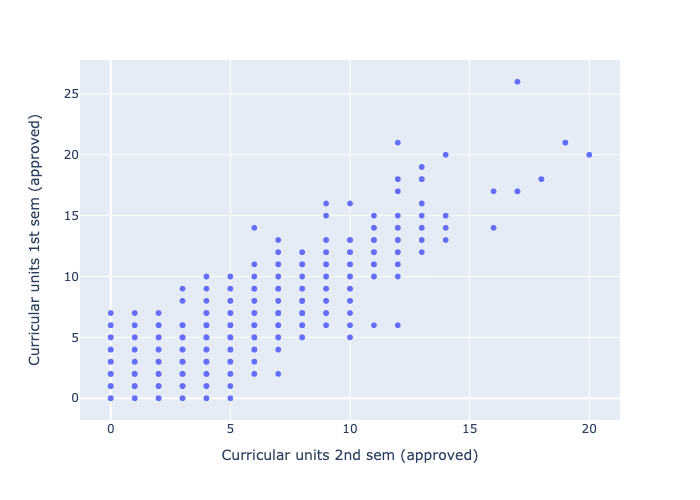
\includegraphics{report_AzadhdhinNedalYunisAlFraijat_files/figure-pdf/cell-47-output-1.png}

We can see that the points for the 1st semester and 2nd semester are
correlated which shows that are one's marks are primary drivers of
success and exhibit sizeable correlations

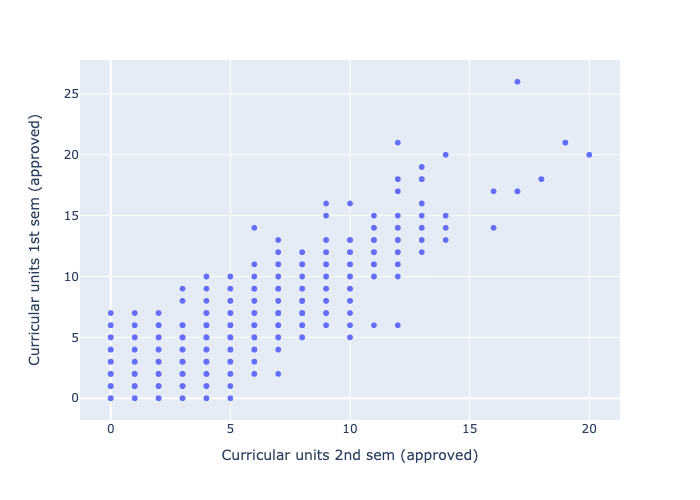
\includegraphics{report_AzadhdhinNedalYunisAlFraijat_files/figure-pdf/cell-48-output-1.png}

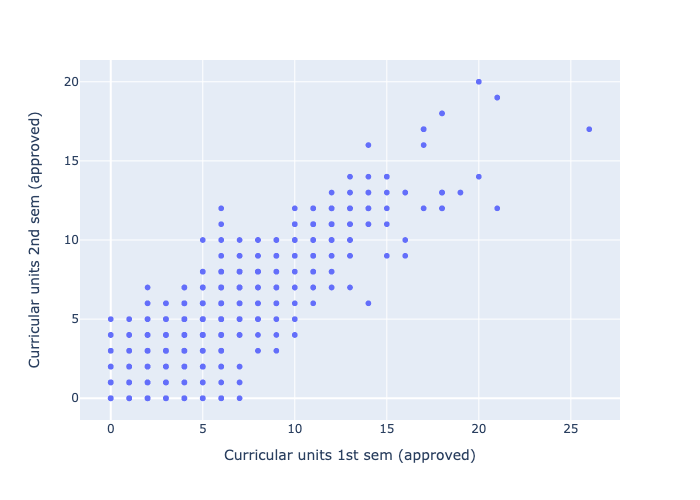
\includegraphics{report_AzadhdhinNedalYunisAlFraijat_files/figure-pdf/cell-49-output-1.png}

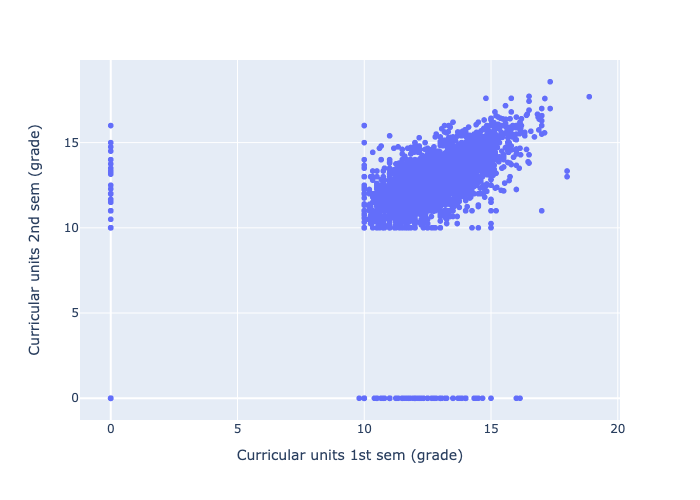
\includegraphics{report_AzadhdhinNedalYunisAlFraijat_files/figure-pdf/cell-50-output-1.png}

\hypertarget{data-mining}{%
\subsection{Data Mining}\label{data-mining}}

\hypertarget{conclusion}{%
\subsection{\texorpdfstring{\textbf{Conclusion}}{Conclusion}}\label{conclusion}}

\begin{quote}
With this analysis, we have some valuable insights some crucial factors
like Academic support, socioeconomic factors, previous qualifications,
and others play a significant role in student retention.
\end{quote}

\begin{quote}
We could work with parents to encourage and support their children's
education. Additionally, We could provide financial assistance to those
who are struggling to pay.
\end{quote}

\begin{quote}
Addressing these factors carefully can effectively lead to dropout rates
reduction and improve overall student outcomes
\end{quote}


\printbibliography


\end{document}
